% ================================================================
% The Retrieve and Connect version of latex/starters/targeted/KS3/algebra/algebraNumberSenseStarters_workedSolutions.tex
%
% This is the same deck as the one above, made by renaming the titles in it.
% Every slide that was a numbered starter is now titled
% "Retrieve and Connect", and the word is renamed wherever else a title
% used it. Nothing outside a title has been changed.
%
%   made from           latex/starters/targeted/KS3/algebra/algebraNumberSenseStarters_workedSolutions.tex
%   retitling rules     version 1
%
% Please don't edit this file. It is written again from the one it was
% made from whenever that changes, so an edit here would be lost - edit
% that file instead and this one follows.
% ================================================================
% Root file used ashow macros
\documentclass{beamer}
\usepackage{tikz}
\usetikzlibrary{calc, arrows.meta, matrix, fit, shapes.geometric}
\usepackage{xcolor}
\usepackage{multicol}
\usepackage{amsmath}
\usepackage{amssymb}

% ================================================================
% Starters for a Year 7 class meeting algebra for the first time, used
% across the algebra unit.
%
% Each starter links an algebraic idea to the number work the class has
% already done, with decimals and negative numbers throughout. Most
% starters open with number calculations that the algebra later on the
% slide uses, and every starter has a sentence to complete with the
% words variable, term, coefficient, constant, expression, equation or
% solution. There are no bar models.
%
%   1  notation: what 3a, ab, a^2 and a/4 mean
%   2  substitution, with whole numbers, decimals and negative numbers
%   3  collecting like terms
%   4  multiplying and dividing terms, and powers
%   5  equations and their solutions, and one-step equations that add
%      or subtract
%   6  one-step equations that multiply or divide
%   7  two-step equations
%   8  two-step equations with decimals and negative numbers
%
% Starters 1 to 4 have no equations. Starters 5 to 8 build up to
% solving two-step equations, and each of them asks pupils to circle the
% reverse of an operation.
%
% The methods follow the ones the class was taught:
%   - Equations are solved by doing the same thing to both sides, never
%     with a flow chart. In the working, a curved arrow on each side goes
%     from one line of the equation to the next, with the operation
%     beside it. Starters 5 to 7 give the operations, and starter 8
%     leaves them blank.
%   - Bus stop division divides a decimal by a whole number, and
%     division by a decimal is done with equivalent fractions, for
%     example 6 / 0.5 = 60 / 5 = 12.
%
% The tables have their first entries filled in, as examples. An
% instruction that belongs to several questions has a bullet, and its
% questions are indented under it. The last question on each starter is
% a challenge, and in starters 1, 2 and 4 the challenge asks whether a
% statement is always, sometimes or never true.
% ================================================================

\setbeamertemplate{navigation symbols}{}
\setbeamersize{text margin left=0.4cm, text margin right=0.4cm}
\setlength{\multicolsep}{2pt}
\setlength{\columnsep}{20pt}

% ================================================================
% Answer-overlay helpers
% ================================================================
\newcommand{\ablank}[1]{%
  \alt<2>{\textcolor{red}{#1}}{\underline{\phantom{#1}}}%
}
\newcommand{\ashow}[1]{\uncover<2->{\textcolor{red}{\small #1}}}
\newcommand{\ashowq}[1]{\alt<2->{\textcolor{red}{\small #1}}{?}}

% Answers drawn straight on to a TikZ diagram, revealed on overlay 2 like \ashow.
% Space is reserved on overlay 1, so the diagram does not move between slides.
\usetikzlibrary{overlay-beamer-styles}
\tikzset{
  ans/.style     = {red, thick, visible on=<2->},
  ansfill/.style = {red!15, visible on=<2->},
  anslab/.style  = {red, font=\tiny, visible on=<2->},
}

% Used by the worked solutions rather than by this deck, so that each worked
% solution is first a question with room to write in and then the answer.
\newlength{\aworkpad}
\setlength{\aworkpad}{8mm}
\newcommand{\awork}[1]{%
  \par\vspace{\aworkpad}%
  \uncover<2->{#1}%
  \par\vspace{\aworkpad}%
}

% Every question list on these slides is tight, so that the diagram column and
% the question column both finish inside the slide.
\newcommand{\tightlist}{%
  \setlength{\itemsep}{0pt}\setlength{\parskip}{0pt}\setlength{\topsep}{0pt}%
}

% An instruction that belongs to several questions: \instr{Solve each
% equation.} puts it beside a bullet, where the question numbers go, and
% the questions in the subqs environment after it are indented under it.
% Their numbers carry on from the questions before them.
\setbeamertemplate{enumerate subitem}{\insertsubenumlabel.}
\renewcommand{\theenumii}{\arabic{enumii}}
\setbeamerfont{itemize/enumerate subbody}{size=\footnotesize}
\setlength{\leftmarginii}{1.4em}
\newcommand{\instr}[1]{%
  \item[{\usebeamercolor[fg]{itemize item}\usebeamertemplate{itemize item}}] #1}
\newenvironment{subqs}
  {\begin{enumerate}\tightlist\setcounter{enumii}{\value{enumi}}}
  {\setcounter{enumi}{\value{enumii}}\end{enumerate}}

% A temperature in degrees Celsius: \dC{-4}.
\newcommand{\dC}[1]{$#1\,^{\circ}$C}

% ================================================================
% The pictures these starters are built from.
% ================================================================
\tikzset{
  dhead/.style = {font=\scriptsize\bfseries, anchor=west},
  vans/.style  = {anslab, font=\scriptsize},
}

% A heading over a table or a picture in the diagram column.
\newcommand{\dheading}[1]{{\scriptsize\bfseries #1}\par\vspace{0.2em}}

% A blank in a table. It is never narrower than 1.6em, so that a one-digit
% answer still leaves a blank that can be seen. \tgiven is an entry that is
% filled in already, as an example, and is the same width.
\newcommand{\tblank}[1]{\ablank{\makebox[1.6em]{#1}}}
\newcommand{\tgiven}[1]{\makebox[1.6em]{#1}}

% Options to circle. \circleops{n}{k} writes +k, -k, \times k and \div k in a
% row, and circles the n-th of them in red on the answer slide. With k empty
% it writes the four signs on their own. The circle takes up no room in the
% line, so the options sit in the same places whichever one is circled, and
% the quads between them keep it clear of its neighbours.
\newcommand{\opt}[1]{\tikz[baseline=(o.base)]\node[inner sep=1.5pt, minimum width=1.6em] (o) {#1};}
\newcommand{\optc}[1]{\tikz[baseline=(o.base)]{%
  \node[inner sep=1.5pt, minimum width=1.6em] (o) {#1};
  \node[ans, draw, ellipse, inner sep=0pt, fit=(o), overlay] {};}}
\newcommand{\circleops}[2]{%
  \ifnum#1=1 \optc{$+#2$}\else\opt{$+#2$}\fi\quad
  \ifnum#1=2 \optc{$-#2$}\else\opt{$-#2$}\fi\quad
  \ifnum#1=3 \optc{$\times#2$}\else\opt{$\times#2$}\fi\quad
  \ifnum#1=4 \optc{$\div#2$}\else\opt{$\div#2$}\fi}

% Solving an equation by doing the same thing to both sides. The lines of the
% equation are the rows of a matrix, lined up on the equals sign, and a curved
% arrow on each side goes from one line to the next, with the operation beside
% it. The operations are a list, one for each step:
%   \bothsides{Working for Q6}{3n+4 \& = \& 19\\ 3n \& = \& \ablank{15}\\
%     n \& = \& \ablank{5}\\}{-4, \div3}
% An operation given as \ablank{...} is left for pupils to write in.
\tikzset{
  bsline/.style  = {matrix of math nodes, ampersand replacement=\&,
                    row sep=0.85em, column sep=0.15em,
                    nodes={inner sep=1pt, font=\footnotesize},
                    column 1/.style={anchor=base east},
                    column 2/.style={anchor=base},
                    column 3/.style={anchor=base west}},
  bsarrow/.style = {-{Stealth[length=3.5pt]}, blue!55!black, semithick},
  bslab/.style   = {font=\scriptsize, text=blue!55!black, inner sep=0.5pt},
}
\newcommand{\bothsides}[3]{%
  \par{\scriptsize\bfseries #1}\par\vspace{0.2em}%
  \begin{tikzpicture}[baseline=(current bounding box.north)]
    \matrix (m) [bsline] {#2};
    \foreach \op [count=\i, evaluate=\i as \j using int(\i+1)] in {#3} {
      \draw[bsarrow] ([xshift=-1pt]m.west |- m-\i-2.center) to[bend right=45]
        node[bslab, left] {$\op$} ([xshift=-1pt]m.west |- m-\j-2.center);
      \draw[bsarrow] ([xshift=1pt]m.east |- m-\i-2.center) to[bend left=45]
        node[bslab, right] {$\op$} ([xshift=1pt]m.east |- m-\j-2.center);
    }
  \end{tikzpicture}\par}

% ---- Bus stop division ----
% The dividend sits on the baseline y = 0 and the answer on y = 0.55, digit
% above digit, with the bus stop drawn between them. A remainder carried to
% the next digit is written small, just before that digit. \busframe{divisor}
% {right end} draws the divisor and the bus stop.
\tikzset{
  bsd/.style     = {font=\footnotesize, inner sep=0pt, anchor=base},
  bsa/.style     = {bsd, red, visible on=<2->},
  bscarry/.style = {font=\tiny, inner sep=0pt, anchor=base, red, visible on=<2->},
}
\newcommand{\busframe}[2]{%
  \node[bsd, anchor=base east] at (-0.1,0) {$#1$};
  \draw[thick] (0,-0.12) -- (0,0.4) -- (#2,0.4);}

% \rect{length}{width}{label in the middle}: a rectangle 2.5 cm by 1.1 cm,
% with its length written above it and its width to its left.
\newcommand{\rect}[3]{%
  \draw[thick, fill=blue!6] (0.9,0) rectangle (3.4,1.1);
  \node[above] at (2.15,1.1) {$#1$};
  \node[left] at (0.9,0.55) {$#2$};
  \node at (2.15,0.55) {#3};}

\title{Algebra \& Number Sense: Retrieve and Connects}
\author{}
\date{}

\begin{document}

\frame{\titlepage}

\begin{frame}{Contents}
\small
\begin{columns}[T]
\begin{column}{0.48\textwidth}
\textbf{Questions and short answers}
\begin{itemize}
\item \hyperlink{q-st1}{\beamergotobutton{Retrieve and Connect 1}}
\item \hyperlink{q-st2}{\beamergotobutton{Retrieve and Connect 2}}
\item \hyperlink{q-st3}{\beamergotobutton{Retrieve and Connect 3}}
\item \hyperlink{q-st4}{\beamergotobutton{Retrieve and Connect 4}}
\item \hyperlink{q-st5}{\beamergotobutton{Retrieve and Connect 5}}
\item \hyperlink{q-st6}{\beamergotobutton{Retrieve and Connect 6}}
\item \hyperlink{q-st7}{\beamergotobutton{Retrieve and Connect 7}}
\item \hyperlink{q-st8}{\beamergotobutton{Retrieve and Connect 8}}
\end{itemize}
\end{column}
\begin{column}{0.48\textwidth}
\textbf{Worked solutions}
\begin{itemize}
\item \hyperlink{work-st1}{\beamergotobutton{Retrieve and Connect 1}}
\item \hyperlink{work-st2}{\beamergotobutton{Retrieve and Connect 2}}
\item \hyperlink{work-st3}{\beamergotobutton{Retrieve and Connect 3}}
\item \hyperlink{work-st4}{\beamergotobutton{Retrieve and Connect 4}}
\item \hyperlink{work-st5}{\beamergotobutton{Retrieve and Connect 5}}
\item \hyperlink{work-st6}{\beamergotobutton{Retrieve and Connect 6}}
\item \hyperlink{work-st7}{\beamergotobutton{Retrieve and Connect 7}}
\item \hyperlink{work-st8}{\beamergotobutton{Retrieve and Connect 8}}
\end{itemize}
\end{column}
\end{columns}
\end{frame}

%------------------------------------------------------------------
% STARTER 1: Algebraic notation. No equations.
%------------------------------------------------------------------
\begin{frame}[t]{Retrieve and Connect: Algebraic Notation}
\hypertarget{q-st1}{}
\begin{columns}[T,onlytextwidth]

\column{0.32\textwidth}
\vspace{-0.4em}
\dheading{Table for Q3}
% --- Q3 answer: the right-hand column. The first row is an example. ---
{\footnotesize
\renewcommand{\arraystretch}{1.25}
\begin{tabular}{@{}l|l@{}}
  With $\times$ or $\div$ & In algebra\\ \hline
  $3\times a$ & \tgiven{$3a$}\\
  $a\times b$ & \tblank{$ab$}\\
  $a\times a$ & \tblank{$a^2$}\\
  $a\div4$    & \tblank{$\dfrac{a}{4}$}\\[2pt]
  $1\times a$ & \tblank{$a$}
\end{tabular}}

\column{0.68\textwidth}
\vspace{-1.5em}
\footnotesize
\begin{enumerate}\tightlist
\begin{multicols}{2}
  \item $3\times(-2)={}$\ashow{$-6$}
  \columnbreak
  \item $3\times0.4={}$\ashow{$1.2$}
\end{multicols}
  \item Write each one in algebra, in the table on the left. The first one
        is done for you.
  \instr{Find the value of $3a$:}
  \begin{subqs}
  {\setlength{\columnsep}{12pt}%
  \begin{multicols}{3}
    \item when $a=5$ \ashow{$15$, not $35$}
    \columnbreak
    \item when $a=0.4$ \ashow{$1.2$}
    \columnbreak
    \item when $a=-2$ \ashow{$-6$}
  \end{multicols}}
  \end{subqs}
  \item In $7y+2$, the $7$ is the \ablank{coefficient}, $y$ is the
        \ablank{variable} and $2$ is the \ablank{constant}.
  \instr{Write an expression for each one.}
  \begin{subqs}
  \begin{multicols}{2}
    \item $n$ multiplied by $4$, then $3$ added \ashow{$4n+3$}
    \columnbreak
    \item $n$ divided by $2$, then $1$ subtracted \ashow{$\tfrac{n}{2}-1$}
  \end{multicols}
  \end{subqs}
  \instr{Is each statement always, sometimes or never true? Try some values
         of $a$ and $b$.}
  \begin{subqs}
    \item (Challenge) $ab$ and $ba$ have the same value.
          \ashow{Always, for example $5\times3=3\times5$.}
    \item (Challenge) $a-b$ and $b-a$ have the same value.
          \ashow{Sometimes: only when $a=b$, because $5-3=2$ but $3-5=-2$.}
  \end{subqs}
\end{enumerate}
\end{columns}
\end{frame}

\begin{frame}[t]{Worked Solution: Retrieve and Connect 1, Question 1}
\hypertarget{work-st1}{}
\textbf{Question:} Work out \(3\times(-2)\).
\awork{\textbf{Solution:} \(3\times(-2)=-6\). A positive number times a negative number is negative.}
\end{frame}

\begin{frame}[t]{Worked Solution: Retrieve and Connect 1, Question 2}
\textbf{Question:} Work out \(3\times0.4\).
\awork{\textbf{Solution:} \(3\times0.4=1.2\).}
\end{frame}

\begin{frame}[t]{Worked Solution: Retrieve and Connect 1, Question 3}
\textbf{Question:} Write each one in algebra: \(3\times a\), \(a\times b\), \(a\times a\), \(a\div4\), \(1\times a\).
\awork{\textbf{Solution:} \(3\times a=3a\), \(a\times b=ab\), \(a\times a=a^2\), \(a\div4=\dfrac{a}{4}\), and \(1\times a=a\).}
\end{frame}

\begin{frame}[t]{Worked Solution: Retrieve and Connect 1, Question 4}
\textbf{Question:} Find the value of \(3a\) when \(a=5\).
\awork{\textbf{Solution:} Substitute \(a=5\): \(3a=3\times5=15\). It is not \(35\).}
\end{frame}

\begin{frame}[t]{Worked Solution: Retrieve and Connect 1, Question 5}
\textbf{Question:} Find the value of \(3a\) when \(a=0.4\).
\awork{\textbf{Solution:} \(3a=3\times0.4=1.2\).}
\end{frame}

\begin{frame}[t]{Worked Solution: Retrieve and Connect 1, Question 6}
\textbf{Question:} Find the value of \(3a\) when \(a=-2\).
\awork{\textbf{Solution:} \(3a=3\times(-2)=-6\).}
\end{frame}

\begin{frame}[t]{Worked Solution: Retrieve and Connect 1, Question 7}
\textbf{Question:} In \(7y+2\), identify the coefficient, the variable and the constant.
\awork{\textbf{Solution:} The coefficient is \(7\), the variable is \(y\), and the constant is \(2\).}
\end{frame}

\begin{frame}[t]{Worked Solution: Retrieve and Connect 1, Question 8}
\textbf{Question:} Write an expression for: \(n\) multiplied by \(4\), then \(3\) added.
\awork{\textbf{Solution:} Multiplying \(n\) by \(4\) gives \(4n\). Adding \(3\) gives \(4n+3\).}
\end{frame}

\begin{frame}[t]{Worked Solution: Retrieve and Connect 1, Question 9}
\textbf{Question:} Write an expression for: \(n\) divided by \(2\), then \(1\) subtracted.
\awork{\textbf{Solution:} Dividing \(n\) by \(2\) gives \(\dfrac{n}{2}\). Subtracting \(1\) gives \(\dfrac{n}{2}-1\).}
\end{frame}

\begin{frame}[t]{Worked Solution: Retrieve and Connect 1, Question 10}
\textbf{Question:} (Challenge) Is it always, sometimes or never true that \(ab\) and \(ba\) have the same value?
\awork{\textbf{Solution:} Always. Multiplication is commutative, so \(ab=ba\). For example, \(5\times3=15=3\times5\).}
\end{frame}

\begin{frame}[t]{Worked Solution: Retrieve and Connect 1, Question 11}
\textbf{Question:} (Challenge) Is it always, sometimes or never true that \(a-b\) and \(b-a\) have the same value?
\awork{\textbf{Solution:} Sometimes. They are equal only when \(a=b\). For example, \(5-3=2\) but \(3-5=-2\).}
\end{frame}

%------------------------------------------------------------------
% STARTER 2: Substitution. No equations.
%------------------------------------------------------------------
\begin{frame}[t]{Retrieve and Connect: Substitution}
\hypertarget{q-st2}{}
\begin{columns}[T,onlytextwidth]

\column{0.32\textwidth}
\vspace{-0.4em}
\dheading{Table for Q4}
% --- Q4 answer: the value of each expression. Three of them are given as
% examples: 2x and x+3 when x = 4, and 5-x when x = 0.5. ---
{\footnotesize
\renewcommand{\arraystretch}{1.3}\setlength{\tabcolsep}{4pt}
\begin{tabular}{@{}c|c|c|c@{}}
  $x$   & $2x$ & $x+3$ & $5-x$\\ \hline
  $4$   & \tgiven{$8$}  & \tgiven{$7$}   & \tblank{$1$}\\
  $0.5$ & \tblank{$1$}  & \tblank{$3.5$} & \tgiven{$4.5$}\\
  $-2$  & \tblank{$-4$} & \tblank{$1$}   & \tblank{$7$}
\end{tabular}}

\column{0.68\textwidth}
\vspace{-1.5em}
\footnotesize
\begin{enumerate}\tightlist
\begin{multicols}{2}
  \item $5-(-2)={}$\ashow{$7$}
  \columnbreak
  \item $4\times(-3)={}$\ashow{$-12$}
\end{multicols}
  \item Replacing a variable with a number is called \ablank{substitution}.
  \item Complete the table on the left. Three of the answers are done for
        you.
  \instr{Find the value of $4a-1$:}
  \begin{subqs}
  \begin{multicols}{2}
    \item when $a=3$ \ashow{$12-1=11$}
    \columnbreak
    \item when $a=-3$ \ashow{$-12-1=-13$}
  \end{multicols}
  \end{subqs}
  \item Find the value of $3x^2$ when $x=2$.
        \ashow{$3\times4=12$. The power comes first, so it is not $6^2$.}
  \item A taxi journey of $m$ miles costs \pounds$(2.5m+3)$. How much does a
        $4$ mile journey cost?
        \ashow{$2.5\times4+3=13$, so \pounds13}
  \item In $2.5m+3$, the coefficient of $m$ is \ablank{$2.5$} and the
        constant is \ablank{$3$}.
  \item (Challenge) Is this statement always, sometimes or never true?
        $2x$ is bigger than $x$.
        \ashow{Sometimes. It is true when $x$ is positive, but when $x=-1$,
        $2x=-2$.}
\end{enumerate}
\end{columns}
\end{frame}

\begin{frame}[t]{Worked Solution: Retrieve and Connect 2, Question 1}
\hypertarget{work-st2}{}
\textbf{Question:} Work out \(5-(-2)\).
\awork{\textbf{Solution:} Subtracting a negative is the same as adding: \(5-(-2)=5+2=7\).}
\end{frame}

\begin{frame}[t]{Worked Solution: Retrieve and Connect 2, Question 2}
\textbf{Question:} Work out \(4\times(-3)\).
\awork{\textbf{Solution:} \(4\times(-3)=-12\).}
\end{frame}

\begin{frame}[t]{Worked Solution: Retrieve and Connect 2, Question 3}
\textbf{Question:} Replacing a variable with a number is called what?
\awork{\textbf{Solution:} It is called substitution.}
\end{frame}

\begin{frame}[t]{Worked Solution: Retrieve and Connect 2, Question 4}
\textbf{Question:} Complete the table of values for \(2x\), \(x+3\) and \(5-x\) at \(x=4,0.5,-2\).
\awork{\textbf{Solution:} The completed table is
\[
\begin{array}{c|c|c|c}
x & 2x & x+3 & 5-x\\ \hline
4 & 8 & 7 & 1\\
0.5 & 1 & 3.5 & 4.5\\
-2 & -4 & 1 & 7
\end{array}
\]}
\end{frame}

\begin{frame}[t]{Worked Solution: Retrieve and Connect 2, Question 5}
\textbf{Question:} Find the value of \(4a-1\) when \(a=3\).
\awork{\textbf{Solution:} \(4a-1=4\times3-1=12-1=11\).}
\end{frame}

\begin{frame}[t]{Worked Solution: Retrieve and Connect 2, Question 6}
\textbf{Question:} Find the value of \(4a-1\) when \(a=-3\).
\awork{\textbf{Solution:} \(4a-1=4\times(-3)-1=-12-1=-13\).}
\end{frame}

\begin{frame}[t]{Worked Solution: Retrieve and Connect 2, Question 7}
\textbf{Question:} Find the value of \(3x^2\) when \(x=2\).
\awork{\textbf{Solution:} The power comes first: \(x^2=2^2=4\). Then \(3x^2=3\times4=12\). It is not \((3\times2)^2=36\).}
\end{frame}

\begin{frame}[t]{Worked Solution: Retrieve and Connect 2, Question 8}
\textbf{Question:} A taxi journey of \(m\) miles costs \pounds\((2.5m+3)\). How much does a \(4\) mile journey cost?
\awork{\textbf{Solution:} Substitute \(m=4\): \(2.5\times4+3=10+3=13\). The cost is \pounds13.}
\end{frame}

\begin{frame}[t]{Worked Solution: Retrieve and Connect 2, Question 9}
\textbf{Question:} In \(2.5m+3\), state the coefficient of \(m\) and the constant.
\awork{\textbf{Solution:} The coefficient of \(m\) is \(2.5\), and the constant is \(3\).}
\end{frame}

\begin{frame}[t]{Worked Solution: Retrieve and Connect 2, Question 10}
\textbf{Question:} (Challenge) Is \(2x\) bigger than \(x\) always, sometimes or never true?
\awork{\textbf{Solution:} Sometimes. It is true when \(x\) is positive, for example \(2\times3=6>3\). But when \(x=-1\), \(2x=-2\), which is not bigger than \(-1\).}
\end{frame}

%------------------------------------------------------------------
% STARTER 3: Collecting like terms. No equations.
%------------------------------------------------------------------
\begin{frame}[t]{Retrieve and Connect: Collecting Like Terms}
\hypertarget{q-st3}{}
\begin{columns}[T,onlytextwidth]

\column{0.32\textwidth}
\vspace{-0.4em}
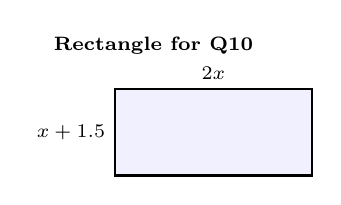
\begin{tikzpicture}[every node/.style={font=\scriptsize}]
\node[dhead] at (0,1.65) {Rectangle for Q10};
\rect{2x}{x+1.5}{}
\end{tikzpicture}

\column{0.68\textwidth}
\vspace{-1.5em}
\footnotesize
\begin{enumerate}\tightlist
  \instr{Work out each calculation, then use it to simplify the expression
         beside it.}
  \begin{subqs}
  \begin{multicols}{2}
    \item $-2+5={}$\ashow{$3$}
    \item $4-9={}$\ashow{$-5$}
    \item $0.3+0.4={}$\ashow{$0.7$}
    \columnbreak
    \item $-2a+5a={}$\ashow{$3a$}
    \item $4y-9y={}$\ashow{$-5y$}
    \item $0.3x+0.4x={}$\ashow{$0.7x$}
  \end{multicols}
  \end{subqs}
  \item $3x$ and $4x$ are called \ablank{like terms}, because only their
        \ablank{coefficients} are different.
  \instr{Simplify each expression.}
  \begin{subqs}
  \begin{multicols}{2}
    \item $5a+2b-3a+b={}$\ashow{$2a+3b$}
    \columnbreak
    \item $1.5m-4+2.5m+6={}$\ashow{$4m+2$}
  \end{multicols}
  \end{subqs}
  \item Write an expression for the perimeter of the rectangle, and simplify it.
        \ashow{$2x+2x+(x+1.5)+(x+1.5)=6x+3$}
  \item Ali simplifies $3x+4y$ to $7xy$. Test this with $x=2$ and $y=10$.
        \ashow{$3x+4y=6+40=46$, but $7xy=140$}
  \item (Challenge) Write an expression with four terms that simplifies to
        $-3x+0.5$.
        \ashow{For example $x-4x+1-0.5$}
\end{enumerate}
\end{columns}
\end{frame}

\begin{frame}[t]{Worked Solution: Retrieve and Connect 3, Question 1}
\hypertarget{work-st3}{}
\textbf{Question:} Work out \(-2+5\).
\awork{\textbf{Solution:} \(-2+5=3\).}
\end{frame}

\begin{frame}[t]{Worked Solution: Retrieve and Connect 3, Question 2}
\textbf{Question:} Work out \(4-9\).
\awork{\textbf{Solution:} \(4-9=-5\).}
\end{frame}

\begin{frame}[t]{Worked Solution: Retrieve and Connect 3, Question 3}
\textbf{Question:} Work out \(0.3+0.4\).
\awork{\textbf{Solution:} \(0.3+0.4=0.7\).}
\end{frame}

\begin{frame}[t]{Worked Solution: Retrieve and Connect 3, Question 4}
\textbf{Question:} Simplify \(-2a+5a\).
\awork{\textbf{Solution:} \(-2a+5a=3a\). The coefficients add: \(-2+5=3\).}
\end{frame}

\begin{frame}[t]{Worked Solution: Retrieve and Connect 3, Question 5}
\textbf{Question:} Simplify \(4y-9y\).
\awork{\textbf{Solution:} \(4y-9y=-5y\). The coefficients subtract: \(4-9=-5\).}
\end{frame}

\begin{frame}[t]{Worked Solution: Retrieve and Connect 3, Question 6}
\textbf{Question:} Simplify \(0.3x+0.4x\).
\awork{\textbf{Solution:} \(0.3x+0.4x=0.7x\).}
\end{frame}

\begin{frame}[t]{Worked Solution: Retrieve and Connect 3, Question 7}
\textbf{Question:} \(3x\) and \(4x\) are called what, because only their coefficients are different?
\awork{\textbf{Solution:} They are called like terms, because only their coefficients are different.}
\end{frame}

\begin{frame}[t]{Worked Solution: Retrieve and Connect 3, Question 8}
\textbf{Question:} Simplify \(5a+2b-3a+b\).
\awork{\textbf{Solution:} Collect the \(a\)-terms and the \(b\)-terms: \(5a-3a=2a\) and \(2b+b=3b\). So the expression is \(2a+3b\).}
\end{frame}

\begin{frame}[t]{Worked Solution: Retrieve and Connect 3, Question 9}
\textbf{Question:} Simplify \(1.5m-4+2.5m+6\).
\awork{\textbf{Solution:} \(1.5m+2.5m=4m\), and \(-4+6=2\). So the expression is \(4m+2\).}
\end{frame}

\begin{frame}[t]{Worked Solution: Retrieve and Connect 3, Question 10}
\textbf{Question:} Write an expression for the perimeter of the rectangle with sides \(2x\) and \(x+1.5\), and simplify it.
\awork{\textbf{Solution:} The perimeter is \(2(2x)+2(x+1.5)=4x+2x+3=6x+3\).}
\end{frame}

\begin{frame}[t]{Worked Solution: Retrieve and Connect 3, Question 11}
\textbf{Question:} Ali simplifies \(3x+4y\) to \(7xy\). Test this with \(x=2\) and \(y=10\).
\awork{\textbf{Solution:} \(3x+4y=3\times2+4\times10=6+40=46\). But \(7xy=7\times2\times10=140\). They are not equal, so Ali is wrong; \(3x\) and \(4y\) are not like terms.}
\end{frame}

\begin{frame}[t]{Worked Solution: Retrieve and Connect 3, Question 12}
\textbf{Question:} (Challenge) Write an expression with four terms that simplifies to \(-3x+0.5\).
\awork{\textbf{Solution:} One example is \(x-4x+1-0.5\). The \(x\)-terms give \(x-4x=-3x\), and the numbers give \(1-0.5=0.5\).}
\end{frame}

%------------------------------------------------------------------
% STARTER 4: Multiplying and dividing terms, and powers. No equations.
%------------------------------------------------------------------
\begin{frame}[t]{Retrieve and Connect: Multiplying Terms \& Powers}
\hypertarget{q-st4}{}
\begin{columns}[T,onlytextwidth]

\column{0.32\textwidth}
\vspace{-0.4em}
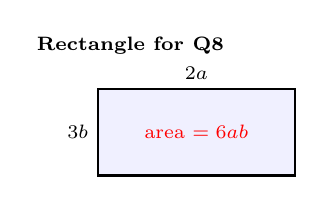
\begin{tikzpicture}[every node/.style={font=\scriptsize}]
\node[dhead] at (0,1.65) {Rectangle for Q8};
\rect{2a}{3b}{}
% --- Q8 answer: the area, written in the rectangle ---
\node[vans] at (2.15,0.55) {area $=6ab$};
\end{tikzpicture}

\vspace{1.2em}
\dheading{Table for Q9}
% --- Q9 answer: the squares. The first one is an example. ---
{\footnotesize
\renewcommand{\arraystretch}{1.3}\setlength{\tabcolsep}{4pt}
\begin{tabular}{@{}c|c|c|c|c@{}}
  $a$   & $3$ & $1$ & $0.5$ & $-2$\\ \hline
  $a^2$ & \tgiven{$9$} & \tblank{$1$} & \tblank{$0.25$} & \tblank{$4$}
\end{tabular}}

\column{0.68\textwidth}
\vspace{-1.5em}
\footnotesize
\begin{enumerate}\tightlist
  \instr{Work out each calculation, then use it to simplify the expression
         beside it.}
  \begin{subqs}
  \begin{multicols}{2}
    \item $-4\times3={}$\ashow{$-12$}
    \item $0.5\times0.5={}$\ashow{$0.25$}
    \columnbreak
    \item $-4\times3a={}$\ashow{$-12a$}
    \item $0.5a\times0.5a={}$\ashow{$0.25a^2$}
  \end{multicols}
  \end{subqs}
  \item In $0.25a^2$, the $0.25$ is the \ablank{coefficient} and the $2$ is
        the \ablank{power}.
  \instr{Simplify each expression.}
  \begin{subqs}
  \begin{multicols}{2}
    \item $4x\times x={}$\ashow{$4x^2$}
    \columnbreak
    \item $-12a\div4={}$\ashow{$-3a$}
  \end{multicols}
  \end{subqs}
  \item Write an expression for the area of the rectangle. Find the area when
        $a=1.5$ and $b=2$.
        \ashow{$2a\times3b=6ab$, \; $6\times1.5\times2=18$}
  \item Complete the table. The first one is done for you. For which value
        of $a$ is $a^2$ smaller than $a$?
        \ashow{$a=0.5$}
  \instr{Find the value of each expression when $a=3$.}
  \begin{subqs}
  \begin{multicols}{2}
    \item $2a^2={}$\ashow{$2\times9=18$}
    \columnbreak
    \item $(2a)^2={}$\ashow{$6^2=36$}
  \end{multicols}
  \end{subqs}
  \item (Challenge) Is this statement always, sometimes or never true?
        $a^2$ is bigger than $a$.
        \ashow{Sometimes. It is not true when $a$ is from $0$ to $1$, for
        example $0.5^2=0.25$.}
\end{enumerate}
\end{columns}
\end{frame}

\begin{frame}[t]{Worked Solution: Retrieve and Connect 4, Question 1}
\hypertarget{work-st4}{}
\textbf{Question:} Work out \(-4\times3\).
\awork{\textbf{Solution:} \(-4\times3=-12\).}
\end{frame}

\begin{frame}[t]{Worked Solution: Retrieve and Connect 4, Question 2}
\textbf{Question:} Work out \(0.5\times0.5\).
\awork{\textbf{Solution:} \(0.5\times0.5=0.25\).}
\end{frame}

\begin{frame}[t]{Worked Solution: Retrieve and Connect 4, Question 3}
\textbf{Question:} Simplify \(-4\times3a\).
\awork{\textbf{Solution:} \(-4\times3a=(-4\times3)a=-12a\).}
\end{frame}

\begin{frame}[t]{Worked Solution: Retrieve and Connect 4, Question 4}
\textbf{Question:} Simplify \(0.5a\times0.5a\).
\awork{\textbf{Solution:} \(0.5a\times0.5a=(0.5\times0.5)(a\times a)=0.25a^2\).}
\end{frame}

\begin{frame}[t]{Worked Solution: Retrieve and Connect 4, Question 5}
\textbf{Question:} In \(0.25a^2\), identify the coefficient and the power.
\awork{\textbf{Solution:} The coefficient is \(0.25\), and the power is \(2\).}
\end{frame}

\begin{frame}[t]{Worked Solution: Retrieve and Connect 4, Question 6}
\textbf{Question:} Simplify \(4x\times x\).
\awork{\textbf{Solution:} \(4x\times x=4x^2\), because \(x\times x=x^2\).}
\end{frame}

\begin{frame}[t]{Worked Solution: Retrieve and Connect 4, Question 7}
\textbf{Question:} Simplify \(-12a\div4\).
\awork{\textbf{Solution:} \(-12a\div4=(-12\div4)a=-3a\).}
\end{frame}

\begin{frame}[t]{Worked Solution: Retrieve and Connect 4, Question 8}
\textbf{Question:} Write an expression for the area of the rectangle with sides \(2a\) and \(3b\). Find the area when \(a=1.5\) and \(b=2\).
\awork{\textbf{Solution:} Area \(=2a\times3b=6ab\). When \(a=1.5\) and \(b=2\), the area is \(6\times1.5\times2=18\).}
\end{frame}

\begin{frame}[t]{Worked Solution: Retrieve and Connect 4, Question 9}
\textbf{Question:} Complete the table of squares, and state for which value of \(a\) in the table \(a^2\) is smaller than \(a\).
\awork{\textbf{Solution:} The completed table is
\[
\begin{array}{c|c|c|c|c}
a & 3 & 1 & 0.5 & -2\\ \hline
a^2 & 9 & 1 & 0.25 & 4
\end{array}
\]
For \(a=0.5\), \(a^2=0.25\), which is smaller than \(0.5\).}
\end{frame}

\begin{frame}[t]{Worked Solution: Retrieve and Connect 4, Question 10}
\textbf{Question:} Find the value of \(2a^2\) when \(a=3\).
\awork{\textbf{Solution:} \(2a^2=2\times3^2=2\times9=18\).}
\end{frame}

\begin{frame}[t]{Worked Solution: Retrieve and Connect 4, Question 11}
\textbf{Question:} Find the value of \((2a)^2\) when \(a=3\).
\awork{\textbf{Solution:} \((2a)^2=(2\times3)^2=6^2=36\).}
\end{frame}

\begin{frame}[t]{Worked Solution: Retrieve and Connect 4, Question 12}
\textbf{Question:} (Challenge) Is \(a^2\) bigger than \(a\) always, sometimes or never true?
\awork{\textbf{Solution:} Sometimes. For example, \(2^2=4>2\), but \(0.5^2=0.25<0.5\). It is equal when \(a=0\) or \(a=1\).}
\end{frame}

%------------------------------------------------------------------
% STARTER 5: Equations and their solutions; adding and subtracting
%------------------------------------------------------------------
\begin{frame}[t]{Retrieve and Connect: Equations \& Solutions}
\hypertarget{q-st5}{}
\begin{columns}[T,onlytextwidth]

\column{0.32\textwidth}
\vspace{-0.4em}
% --- Q10 answer: x = -4 ---
\bothsides{Working for Q10}{x+7 \& = \& 3\\ x \& = \& \ablank{-4}\\}{-7}

\column{0.68\textwidth}
\vspace{-1.5em}
\footnotesize
\begin{enumerate}\tightlist
\begin{multicols}{2}
  \item $3-7={}$\ashow{$-4$}
  \columnbreak
  \item $1-2.5={}$\ashow{$-1.5$}
\end{multicols}
  \instr{Is each one an expression or an equation?}
  \begin{subqs}
  {\setlength{\columnsep}{12pt}%
  \begin{multicols}{3}
    \item $4x+1$ \ashow{expression}
    \columnbreak
    \item $4x+1=9$ \ashow{equation}
    \columnbreak
    \item $9=x-3$ \ashow{equation}
  \end{multicols}}
  \end{subqs}
  \item A value of $x$ that makes an equation true is called a
        \ablank{solution}.
  \item Is $x=2$ a solution of $4x+1=9$?
        \ashow{Yes, because $4\times2+1=9$}
  \instr{Circle the operation that is the reverse of:}
  \begin{subqs}
    \item \makebox[2.2cm][l]{addition} \circleops{2}{}
    \item \makebox[2.2cm][l]{subtraction} \circleops{1}{}
  \end{subqs}
  \item Solve $x+7=3$, using the working on the left.
  \instr{Solve each equation.}
  \begin{subqs}
  \begin{multicols}{2}
    \item $x-5=-2$ \ashow{$x=3$}
    \columnbreak
    \item $x+2.5=1$ \ashow{$x=-1.5$}
  \end{multicols}
  \end{subqs}
  \item The temperature rose by \dC{6} to \dC{-2}. Solve an equation to find
        the temperature before, $t$.
        \ashow{$t+6=-2$, \; $t=-8$}
  \item (Challenge) Write an equation like $x+7=3$ whose solution is
        $x=-2.5$.
        \ashow{For example $x+4=1.5$}
\end{enumerate}
\end{columns}
\end{frame}

\begin{frame}[t]{Worked Solution: Retrieve and Connect 5, Question 1}
\hypertarget{work-st5}{}
\textbf{Question:} Work out \(3-7\).
\awork{\textbf{Solution:} \(3-7=-4\).}
\end{frame}

\begin{frame}[t]{Worked Solution: Retrieve and Connect 5, Question 2}
\textbf{Question:} Work out \(1-2.5\).
\awork{\textbf{Solution:} \(1-2.5=-1.5\).}
\end{frame}

\begin{frame}[t]{Worked Solution: Retrieve and Connect 5, Question 3}
\textbf{Question:} Is \(4x+1\) an expression or an equation?
\awork{\textbf{Solution:} It is an expression, because it has no equals sign.}
\end{frame}

\begin{frame}[t]{Worked Solution: Retrieve and Connect 5, Question 4}
\textbf{Question:} Is \(4x+1=9\) an expression or an equation?
\awork{\textbf{Solution:} It is an equation, because it contains an equals sign.}
\end{frame}

\begin{frame}[t]{Worked Solution: Retrieve and Connect 5, Question 5}
\textbf{Question:} Is \(9=x-3\) an expression or an equation?
\awork{\textbf{Solution:} It is an equation, because it contains an equals sign.}
\end{frame}

\begin{frame}[t]{Worked Solution: Retrieve and Connect 5, Question 6}
\textbf{Question:} A value of \(x\) that makes an equation true is called what?
\awork{\textbf{Solution:} It is called a solution.}
\end{frame}

\begin{frame}[t]{Worked Solution: Retrieve and Connect 5, Question 7}
\textbf{Question:} Is \(x=2\) a solution of \(4x+1=9\)?
\awork{\textbf{Solution:} Substitute \(x=2\): \(4\times2+1=8+1=9\). This is true, so \(x=2\) is a solution.}
\end{frame}

\begin{frame}[t]{Worked Solution: Retrieve and Connect 5, Question 8}
\textbf{Question:} Circle the operation that is the reverse of addition.
\awork{\textbf{Solution:} The reverse of addition is subtraction.}
\end{frame}

\begin{frame}[t]{Worked Solution: Retrieve and Connect 5, Question 9}
\textbf{Question:} Circle the operation that is the reverse of subtraction.
\awork{\textbf{Solution:} The reverse of subtraction is addition.}
\end{frame}

\begin{frame}[t]{Worked Solution: Retrieve and Connect 5, Question 10}
\textbf{Question:} Solve \(x+7=3\), using the working on the left.
\awork{\textbf{Solution:} Subtract \(7\) from both sides: \(x+7-7=3-7\), so \(x=-4\).}
\end{frame}

\begin{frame}[t]{Worked Solution: Retrieve and Connect 5, Question 11}
\textbf{Question:} Solve \(x-5=-2\).
\awork{\textbf{Solution:} Add \(5\) to both sides: \(x-5+5=-2+5\), so \(x=3\).}
\end{frame}

\begin{frame}[t]{Worked Solution: Retrieve and Connect 5, Question 12}
\textbf{Question:} Solve \(x+2.5=1\).
\awork{\textbf{Solution:} Subtract \(2.5\) from both sides: \(x=1-2.5=-1.5\).}
\end{frame}

\begin{frame}[t]{Worked Solution: Retrieve and Connect 5, Question 13}
\textbf{Question:} The temperature rose by \(6^\circ\)C to \(-2^\circ\)C. Solve an equation to find the temperature before, \(t\).
\awork{\textbf{Solution:} The temperature before plus \(6\) equals \(-2\), so \(t+6=-2\). Subtract \(6\): \(t=-2-6=-8\). The temperature before was \(-8^\circ\)C.}
\end{frame}

\begin{frame}[t]{Worked Solution: Retrieve and Connect 5, Question 14}
\textbf{Question:} (Challenge) Write an equation like \(x+7=3\) whose solution is \(x=-2.5\).
\awork{\textbf{Solution:} One example is \(x+4=1.5\), because \(-2.5+4=1.5\).}
\end{frame}

%------------------------------------------------------------------
% STARTER 6: One-step equations that multiply or divide
%------------------------------------------------------------------
\begin{frame}[t]{Retrieve and Connect: One-Step Equations}
\hypertarget{q-st6}{}
\begin{columns}[T,onlytextwidth]

\column{0.32\textwidth}
\vspace{-0.4em}
% --- Q5 answer: x = 0.7 ---
\bothsides{Working for Q5}{4x \& = \& 2.8\\ x \& = \& \ablank{0.7}\\}{\div4}

\vspace{1em}
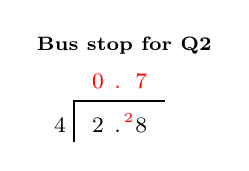
\begin{tikzpicture}[every node/.style={font=\scriptsize}]
% ---- Bus stop division for 2.8 / 4 ----
\begin{scope}[xshift=0.6cm]
\node[dhead] at (-0.6,1.1) {Bus stop for Q2};
\busframe{4}{1.15}
\foreach \x/\d in {0.3/2, 0.55/., 0.85/8} \node[bsd] at (\x,0) {$\d$};
% --- Q2 answer: 2.8 / 4 = 0.7, carrying 2 ---
\foreach \x/\d in {0.3/0, 0.55/., 0.85/7} \node[bsa] at (\x,0.55) {$\d$};
\node[bscarry] at ({0.85-0.16},0.12) {$2$};
\end{scope}
\end{tikzpicture}

\column{0.68\textwidth}
\vspace{-1.5em}
\footnotesize
\begin{enumerate}\tightlist
  \instr{Work out each calculation, then use it to solve the equation
         beside it.}
  \begin{subqs}
  \begin{multicols}{2}
    \item $-18\div3={}$\ashow{$-6$}
    \item $2.8\div4={}$\ashow{$0.7$}
    \item $6\div0.5={}$\ashow{$\tfrac{60}{5}=12$}
    \columnbreak
    \item $3x=-18$ \ashow{$x=-6$}
    \item $4x=2.8$ \ashow{$x=0.7$}
    \item $0.5x=6$ \ashow{$x=12$}
  \end{multicols}
  \end{subqs}
  \item In $4x=2.8$, the $4$ is the \ablank{coefficient} of $x$.
  \instr{Circle the operation that is the reverse of:}
  \begin{subqs}
    \item \makebox[2.2cm][l]{multiplication} \circleops{4}{}
    \item \makebox[2.2cm][l]{division} \circleops{3}{}
  \end{subqs}
  \instr{Solve each equation.}
  \begin{subqs}
  \begin{multicols}{2}
    \item $-2x=10$ \ashow{$x=-5$}
    \columnbreak
    \item $\dfrac{x}{5}=-2$ \ashow{$x=-10$}
  \end{multicols}
  \end{subqs}
  \item Five friends share a bill equally, and each pays \pounds7.40. Solve
        an equation to find the bill, \pounds$b$.
        \ashow{$\tfrac{b}{5}=7.40$, \; $b=37$}
  \instr{Write an equation with the solution $x=-0.5$:}
  \begin{subqs}
  \begin{multicols}{2}
    \item (Challenge) where $x$ is multiplied by a number
          \ashow{For example $4x=-2$}
    \columnbreak
    \item (Challenge) where $x$ is divided by a number
          \ashow{For example $\tfrac{x}{2}=-0.25$}
  \end{multicols}
  \end{subqs}
\end{enumerate}
\end{columns}
\end{frame}

\begin{frame}[t]{Worked Solution: Retrieve and Connect 6, Question 1}
\hypertarget{work-st6}{}
\textbf{Question:} Work out \(-18\div3\).
\awork{\textbf{Solution:} \(-18\div3=-6\).}
\end{frame}

\begin{frame}[t]{Worked Solution: Retrieve and Connect 6, Question 2}
\textbf{Question:} Work out \(2.8\div4\).
\awork{\textbf{Solution:} \(2.8\div4=0.7\), as shown by the bus stop division on the starter.}
\end{frame}

\begin{frame}[t]{Worked Solution: Retrieve and Connect 6, Question 3}
\textbf{Question:} Work out \(6\div0.5\).
\awork{\textbf{Solution:} Dividing by \(0.5\) is the same as multiplying by \(2\). Using equivalent fractions, \(6\div0.5=\dfrac{6}{0.5}=\dfrac{60}{5}=12\).}
\end{frame}

\begin{frame}[t]{Worked Solution: Retrieve and Connect 6, Question 4}
\textbf{Question:} Solve \(3x=-18\).
\awork{\textbf{Solution:} Divide both sides by \(3\): \(x=-18\div3=-6\).}
\end{frame}

\begin{frame}[t]{Worked Solution: Retrieve and Connect 6, Question 5}
\textbf{Question:} Solve \(4x=2.8\), using the working on the left.
\awork{\textbf{Solution:} Divide both sides by \(4\): \(x=2.8\div4=0.7\).}
\end{frame}

\begin{frame}[t]{Worked Solution: Retrieve and Connect 6, Question 6}
\textbf{Question:} Solve \(0.5x=6\).
\awork{\textbf{Solution:} Divide both sides by \(0.5\), which is the same as multiplying by \(2\): \(x=6\div0.5=12\).}
\end{frame}

\begin{frame}[t]{Worked Solution: Retrieve and Connect 6, Question 7}
\textbf{Question:} In \(4x=2.8\), what is the coefficient of \(x\)?
\awork{\textbf{Solution:} The coefficient of \(x\) is \(4\).}
\end{frame}

\begin{frame}[t]{Worked Solution: Retrieve and Connect 6, Question 8}
\textbf{Question:} Circle the operation that is the reverse of multiplication.
\awork{\textbf{Solution:} The reverse of multiplication is division.}
\end{frame}

\begin{frame}[t]{Worked Solution: Retrieve and Connect 6, Question 9}
\textbf{Question:} Circle the operation that is the reverse of division.
\awork{\textbf{Solution:} The reverse of division is multiplication.}
\end{frame}

\begin{frame}[t]{Worked Solution: Retrieve and Connect 6, Question 10}
\textbf{Question:} Solve \(-2x=10\).
\awork{\textbf{Solution:} Divide both sides by \(-2\): \(x=10\div(-2)=-5\).}
\end{frame}

\begin{frame}[t]{Worked Solution: Retrieve and Connect 6, Question 11}
\textbf{Question:} Solve \(\dfrac{x}{5}=-2\).
\awork{\textbf{Solution:} Multiply both sides by \(5\): \(x=-2\times5=-10\).}
\end{frame}

\begin{frame}[t]{Worked Solution: Retrieve and Connect 6, Question 12}
\textbf{Question:} Five friends share a bill equally, and each pays \pounds7.40. Solve an equation to find the bill, \pounds\(b\).
\awork{\textbf{Solution:} Each person pays \(\dfrac{b}{5}\), so \(\dfrac{b}{5}=7.40\). Multiply both sides by \(5\): \(b=7.40\times5=37\). The bill is \pounds37.}
\end{frame}

\begin{frame}[t]{Worked Solution: Retrieve and Connect 6, Question 13}
\textbf{Question:} (Challenge) Write an equation with solution \(x=-0.5\) where \(x\) is multiplied by a number.
\awork{\textbf{Solution:} One example is \(4x=-2\), because \(4\times(-0.5)=-2\).}
\end{frame}

\begin{frame}[t]{Worked Solution: Retrieve and Connect 6, Question 14}
\textbf{Question:} (Challenge) Write an equation with solution \(x=-0.5\) where \(x\) is divided by a number.
\awork{\textbf{Solution:} One example is \(\dfrac{x}{2}=-0.25\), because \(-0.5\div2=-0.25\).}
\end{frame}

%------------------------------------------------------------------
% STARTER 7: Two-step equations, with the operations given
%------------------------------------------------------------------
\begin{frame}[t]{Retrieve and Connect: Two-Step Equations}
\hypertarget{q-st7}{}
\begin{columns}[T,onlytextwidth]

\column{0.32\textwidth}
\vspace{-0.4em}
% --- Q6 answer: the right-hand side of each line ---
\bothsides{Working for Q6}{3n+4 \& = \& 19\\ 3n \& = \& \ablank{15}\\
  n \& = \& \ablank{5}\\}{-4, \div3}

\vspace{0.8em}
% --- Q10 answer: the right-hand side of each line ---
\bothsides{Working for Q10}{4x+9 \& = \& 1\\ 4x \& = \& \ablank{-8}\\
  x \& = \& \ablank{-2}\\}{-9, \div4}

\column{0.68\textwidth}
\vspace{-1.5em}
\footnotesize
\begin{enumerate}\tightlist
\begin{multicols}{2}
  \item $1-9={}$\ashow{$-8$}
  \columnbreak
  \item $-8\div4={}$\ashow{$-2$}
\end{multicols}
  \item In $3n+4=19$, the left-hand side is an \ablank{expression}.
  \instr{Circle the operation that is the reverse of:}
  \begin{subqs}
    \item \makebox[2.6cm][l]{adding $4$} \circleops{2}{4}
    \item \makebox[2.6cm][l]{multiplying by $3$} \circleops{4}{3}
  \end{subqs}
  \item I think of a number, $n$. I multiply it by $3$ and add $4$, and I
        get $19$. Write an equation, then complete the working on the left.
        \ashow{$3n+4=19$}
  \item Check your answer to Q6 by substituting it into $3n+4$.
        \ashow{$3\times5+4=19$ \checkmark}
  \instr{Solve each equation.}
  \begin{subqs}
  \begin{multicols}{2}
    \item $2x+5=11$ \ashow{$2x=6$, \; $x=3$}
    \columnbreak
    \item $5x-3=17$ \ashow{$5x=20$, \; $x=4$}
  \end{multicols}
  \begin{multicols}{2}
    \item $4x+9=1$, with the working on the left
    \columnbreak
    \item $2x-1=6$ \ashow{$2x=7$, \; $x=3.5$}
  \end{multicols}
  \end{subqs}
  \item A plumber charges a \pounds20 call-out fee and \pounds35 an hour. A
        bill is \pounds125. Solve an equation to find the number of hours,
        $h$.
        \ashow{$35h+20=125$, \; $h=3$}
  \item (Challenge) Solve $x+2x+3=18$.
        \ashow{$3x+3=18$, \; $x=5$}
\end{enumerate}
\end{columns}
\end{frame}

\begin{frame}[t]{Worked Solution: Retrieve and Connect 7, Question 1}
\hypertarget{work-st7}{}
\textbf{Question:} Work out \(1-9\).
\awork{\textbf{Solution:} \(1-9=-8\).}
\end{frame}

\begin{frame}[t]{Worked Solution: Retrieve and Connect 7, Question 2}
\textbf{Question:} Work out \(-8\div4\).
\awork{\textbf{Solution:} \(-8\div4=-2\).}
\end{frame}

\begin{frame}[t]{Worked Solution: Retrieve and Connect 7, Question 3}
\textbf{Question:} In \(3n+4=19\), what is the left-hand side called?
\awork{\textbf{Solution:} The left-hand side, \(3n+4\), is an expression.}
\end{frame}

\begin{frame}[t]{Worked Solution: Retrieve and Connect 7, Question 4}
\textbf{Question:} Circle the operation that is the reverse of adding \(4\).
\awork{\textbf{Solution:} The reverse of adding \(4\) is subtracting \(4\).}
\end{frame}

\begin{frame}[t]{Worked Solution: Retrieve and Connect 7, Question 5}
\textbf{Question:} Circle the operation that is the reverse of multiplying by \(3\).
\awork{\textbf{Solution:} The reverse of multiplying by \(3\) is dividing by \(3\).}
\end{frame}

\begin{frame}[t]{Worked Solution: Retrieve and Connect 7, Question 6}
\textbf{Question:} I think of a number \(n\). I multiply it by \(3\) and add \(4\), and I get \(19\). Write an equation, then complete the working.
\awork{\textbf{Solution:} The equation is \(3n+4=19\). Subtract \(4\) from both sides: \(3n=15\). Divide both sides by \(3\): \(n=5\).}
\end{frame}

\begin{frame}[t]{Worked Solution: Retrieve and Connect 7, Question 7}
\textbf{Question:} Check your answer to Q6 by substituting it into \(3n+4\).
\awork{\textbf{Solution:} Substitute \(n=5\): \(3\times5+4=15+4=19\), which matches the equation.}
\end{frame}

\begin{frame}[t]{Worked Solution: Retrieve and Connect 7, Question 8}
\textbf{Question:} Solve \(2x+5=11\).
\awork{\textbf{Solution:} Subtract \(5\) from both sides: \(2x=6\). Divide both sides by \(2\): \(x=3\).}
\end{frame}

\begin{frame}[t]{Worked Solution: Retrieve and Connect 7, Question 9}
\textbf{Question:} Solve \(5x-3=17\).
\awork{\textbf{Solution:} Add \(3\) to both sides: \(5x=20\). Divide both sides by \(5\): \(x=4\).}
\end{frame}

\begin{frame}[t]{Worked Solution: Retrieve and Connect 7, Question 10}
\textbf{Question:} Solve \(4x+9=1\), using the working on the left.
\awork{\textbf{Solution:} Subtract \(9\) from both sides: \(4x=-8\). Divide both sides by \(4\): \(x=-2\).}
\end{frame}

\begin{frame}[t]{Worked Solution: Retrieve and Connect 7, Question 11}
\textbf{Question:} Solve \(2x-1=6\).
\awork{\textbf{Solution:} Add \(1\) to both sides: \(2x=7\). Divide both sides by \(2\): \(x=3.5\).}
\end{frame}

\begin{frame}[t]{Worked Solution: Retrieve and Connect 7, Question 12}
\textbf{Question:} A plumber charges a \pounds20 call-out fee and \pounds35 an hour. A bill is \pounds125. Solve an equation to find the number of hours, \(h\).
\awork{\textbf{Solution:} The cost is \(35h+20\), so \(35h+20=125\). Subtract \(20\): \(35h=105\). Divide by \(35\): \(h=3\). The plumber worked \(3\) hours.}
\end{frame}

\begin{frame}[t]{Worked Solution: Retrieve and Connect 7, Question 13}
\textbf{Question:} (Challenge) Solve \(x+2x+3=18\).
\awork{\textbf{Solution:} Combine like terms: \(x+2x=3x\), so \(3x+3=18\). Subtract \(3\): \(3x=15\). Divide by \(3\): \(x=5\).}
\end{frame}

%------------------------------------------------------------------
% STARTER 8: Two-step equations with decimals and negative numbers,
% with the operations left blank
%------------------------------------------------------------------
\begin{frame}[t]{Retrieve and Connect: Decimals \& Negatives in Equations}
\hypertarget{q-st8}{}
\begin{columns}[T,onlytextwidth]

\column{0.34\textwidth}
\vspace{-0.4em}
% --- Q6 answer: the operations, and the right-hand side of each line ---
\bothsides{Working for Q6}{2x-1.2 \& = \& 3\\ 2x \& = \& \ablank{4.2}\\
  x \& = \& \ablank{2.1}\\}{\ablank{+1.2}, \ablank{\div2}}

\vspace{1.2em}
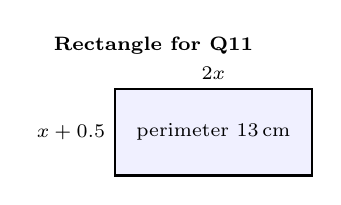
\begin{tikzpicture}[every node/.style={font=\scriptsize}]
\node[dhead] at (0,1.65) {Rectangle for Q11};
\rect{2x}{x+0.5}{perimeter $13$\,cm}
\end{tikzpicture}

\column{0.66\textwidth}
\vspace{-1.5em}
\footnotesize
\begin{enumerate}\tightlist
\begin{multicols}{2}
  \item $3+1.2={}$\ashow{$4.2$}
  \columnbreak
  \item $4.2\div2={}$\ashow{$2.1$}
\end{multicols}
  \item In $2x-1.2=3$, the coefficient of $x$ is \ablank{$2$}, and the
        constant on the left-hand side is \ablank{$-1.2$}.
  \instr{Circle the operation that is the reverse of:}
  \begin{subqs}
    \item \makebox[2.3cm][l]{subtracting $1.2$} \circleops{1}{1.2}
    \item \makebox[2.3cm][l]{multiplying by $2$} \circleops{4}{2}
  \end{subqs}
  \item Solve $2x-1.2=3$. Write the operations beside the arrows.
  \instr{Solve each equation.}
  \begin{subqs}
  \begin{multicols}{2}
    \item $3x+8=-7$ \ashow{$3x=-15$, \; $x=-5$}
    \columnbreak
    \item $\dfrac{x}{2}+3=-1$ \ashow{$\tfrac{x}{2}=-4$, \; $x=-8$}
  \end{multicols}
  \begin{multicols}{2}
    \item $5x-2.5=10$ \ashow{$5x=12.5$, \; $x=2.5$}
    \columnbreak
    \item $0.5x+4=1$
          \ashow{$0.5x=-3$, \; $x=\tfrac{-3}{0.5}=\tfrac{-30}{5}=-6$}
  \end{multicols}
  \end{subqs}
  \item Write an equation for the perimeter of the rectangle, and solve it.
        \ashow{$6x+1=13$, \; $x=2$}
  \item (Challenge) Write a two-step equation with the solution $x=-0.5$.
        \ashow{For example $2x+3=2$}
\end{enumerate}
\end{columns}
\end{frame}

\begin{frame}[t]{Worked Solution: Retrieve and Connect 8, Question 1}
\hypertarget{work-st8}{}
\textbf{Question:} Work out \(3+1.2\).
\awork{\textbf{Solution:} \(3+1.2=4.2\).}
\end{frame}

\begin{frame}[t]{Worked Solution: Retrieve and Connect 8, Question 2}
\textbf{Question:} Work out \(4.2\div2\).
\awork{\textbf{Solution:} \(4.2\div2=2.1\).}
\end{frame}

\begin{frame}[t]{Worked Solution: Retrieve and Connect 8, Question 3}
\textbf{Question:} In \(2x-1.2=3\), state the coefficient of \(x\) and the constant on the left-hand side.
\awork{\textbf{Solution:} The coefficient of \(x\) is \(2\), and the constant on the left-hand side is \(-1.2\).}
\end{frame}

\begin{frame}[t]{Worked Solution: Retrieve and Connect 8, Question 4}
\textbf{Question:} Circle the operation that is the reverse of subtracting \(1.2\).
\awork{\textbf{Solution:} The reverse of subtracting \(1.2\) is adding \(1.2\).}
\end{frame}

\begin{frame}[t]{Worked Solution: Retrieve and Connect 8, Question 5}
\textbf{Question:} Circle the operation that is the reverse of multiplying by \(2\).
\awork{\textbf{Solution:} The reverse of multiplying by \(2\) is dividing by \(2\).}
\end{frame}

\begin{frame}[t]{Worked Solution: Retrieve and Connect 8, Question 6}
\textbf{Question:} Solve \(2x-1.2=3\). Write the operations beside the arrows.
\awork{\textbf{Solution:} Add \(1.2\) to both sides: \(2x=3+1.2=4.2\). Divide both sides by \(2\): \(x=4.2\div2=2.1\).}
\end{frame}

\begin{frame}[t]{Worked Solution: Retrieve and Connect 8, Question 7}
\textbf{Question:} Solve \(3x+8=-7\).
\awork{\textbf{Solution:} Subtract \(8\) from both sides: \(3x=-7-8=-15\). Divide both sides by \(3\): \(x=-5\).}
\end{frame}

\begin{frame}[t]{Worked Solution: Retrieve and Connect 8, Question 8}
\textbf{Question:} Solve \(\dfrac{x}{2}+3=-1\).
\awork{\textbf{Solution:} Subtract \(3\) from both sides: \(\dfrac{x}{2}=-1-3=-4\). Multiply both sides by \(2\): \(x=-8\).}
\end{frame}

\begin{frame}[t]{Worked Solution: Retrieve and Connect 8, Question 9}
\textbf{Question:} Solve \(5x-2.5=10\).
\awork{\textbf{Solution:} Add \(2.5\) to both sides: \(5x=10+2.5=12.5\). Divide both sides by \(5\): \(x=12.5\div5=2.5\).}
\end{frame}

\begin{frame}[t]{Worked Solution: Retrieve and Connect 8, Question 10}
\textbf{Question:} Solve \(0.5x+4=1\).
\awork{\textbf{Solution:} Subtract \(4\) from both sides: \(0.5x=1-4=-3\). Divide both sides by \(0.5\): \(x=\dfrac{-3}{0.5}=\dfrac{-30}{5}=-6\).}
\end{frame}

\begin{frame}[t]{Worked Solution: Retrieve and Connect 8, Question 11}
\textbf{Question:} Write an equation for the perimeter of the rectangle with sides \(2x\) and \(x+0.5\), given that the perimeter is \(13\) cm, and solve it.
\awork{\textbf{Solution:} The perimeter is \(2(2x)+2(x+0.5)=4x+2x+1=6x+1\). So \(6x+1=13\). Subtract \(1\): \(6x=12\). Divide by \(6\): \(x=2\).}
\end{frame}

\begin{frame}[t]{Worked Solution: Retrieve and Connect 8, Question 12}
\textbf{Question:} (Challenge) Write a two-step equation with the solution \(x=-0.5\).
\awork{\textbf{Solution:} One example is \(2x+3=2\), because \(2\times(-0.5)+3=-1+3=2\).}
\end{frame}

\end{document}